\documentclass[11pt,aspectratio=169]{beamer}
\usetheme{Madrid}

% ======================= PACKAGES =======================
\usepackage{graphicx}
\usepackage{booktabs}
\usepackage{adjustbox}
\usepackage{multicol}
\usepackage{amsmath}
\usepackage{amssymb}
\usepackage{tikz}
\usetikzlibrary{arrows,shapes,positioning,shadows,trees}
\usepackage{listings}
\usepackage{xcolor}

% ======================= COLOR DEFINITIONS =======================
% Primary color scheme: Blue/Teal for Digital Finance
\definecolor{dfblue}{RGB}{0,102,204}
\definecolor{dfteal}{RGB}{0,153,153}
\definecolor{dfcyan}{RGB}{51,187,204}
\definecolor{dflightblue}{RGB}{153,204,255}
\definecolor{dflightblue2}{RGB}{173,214,255}
\definecolor{dflightblue3}{RGB}{193,224,255}
\definecolor{dflightblue4}{RGB}{213,234,255}

% Accent colors for finance applications
\definecolor{dfgreen}{RGB}{44, 160, 44}
\definecolor{dfred}{RGB}{214, 39, 40}
\definecolor{dforange}{RGB}{255, 127, 14}
\definecolor{dfgray}{RGB}{127, 127, 127}

% Utility colors
\definecolor{lightgray}{RGB}{240, 240, 240}
\definecolor{midgray}{RGB}{180, 180, 180}
\definecolor{codebg}{RGB}{245, 245, 245}

% ======================= THEME CUSTOMIZATION =======================
% Apply Digital Finance color scheme to Madrid theme
\setbeamercolor{palette primary}{bg=dflightblue3,fg=dfblue}
\setbeamercolor{palette secondary}{bg=dflightblue2,fg=dfblue}
\setbeamercolor{palette tertiary}{bg=dfteal,fg=white}
\setbeamercolor{palette quaternary}{bg=dfblue,fg=white}

\setbeamercolor{structure}{fg=dfblue}
\setbeamercolor{section in toc}{fg=dfblue}
\setbeamercolor{subsection in toc}{fg=dfteal}
\setbeamercolor{title}{fg=dfblue}
\setbeamercolor{frametitle}{fg=dfblue,bg=dflightblue3}
\setbeamercolor{block title}{bg=dflightblue2,fg=dfblue}
\setbeamercolor{block body}{bg=dflightblue4,fg=black}

% Remove navigation symbols for cleaner look
\setbeamertemplate{navigation symbols}{}

% Clean itemize/enumerate
\setbeamertemplate{itemize items}[circle]
\setbeamertemplate{enumerate items}[default]

% Margins for readability
\setbeamersize{text margin left=8mm,text margin right=8mm}

% ======================= LISTINGS CONFIGURATION =======================
% Python code style
\lstdefinestyle{pythonstyle}{
    language=Python,
    basicstyle=\ttfamily\footnotesize,
    keywordstyle=\color{dfblue}\bfseries,
    stringstyle=\color{dforange},
    commentstyle=\color{dfgray}\itshape,
    numberstyle=\tiny\color{dfgray},
    numbers=left,
    numbersep=5pt,
    backgroundcolor=\color{codebg},
    showspaces=false,
    showstringspaces=false,
    showtabs=false,
    frame=single,
    rulecolor=\color{midgray},
    tabsize=4,
    captionpos=b,
    breaklines=true,
    breakatwhitespace=false,
    escapeinside={(*@}{@*)},
    xleftmargin=10pt,
    xrightmargin=10pt
}

% Solidity code style
\lstdefinestyle{soliditystyle}{
    language=Java, % closest approximation
    basicstyle=\ttfamily\footnotesize,
    keywordstyle=\color{dfteal}\bfseries,
    stringstyle=\color{dforange},
    commentstyle=\color{dfgray}\itshape,
    numberstyle=\tiny\color{dfgray},
    numbers=left,
    numbersep=5pt,
    backgroundcolor=\color{codebg},
    showspaces=false,
    showstringspaces=false,
    showtabs=false,
    frame=single,
    rulecolor=\color{midgray},
    tabsize=2,
    captionpos=b,
    breaklines=true,
    breakatwhitespace=false,
    escapeinside={(*@}{@*)},
    xleftmargin=10pt,
    xrightmargin=10pt,
    morekeywords={pragma, contract, function, returns, public, private, view, pure, payable, address, uint256, mapping, event, modifier}
}

% Inline code command
\newcommand{\code}[1]{\texttt{\color{dfblue}#1}}

% ======================= CUSTOM COMMANDS =======================
% Bottom annotation (Madrid-style)
\newcommand{\bottomnote}[1]{%
\vfill
\vspace{-2mm}
\textcolor{dflightblue2}{\rule{\textwidth}{0.4pt}}
\vspace{1mm}
\footnotesize
\textbf{#1}
}

% Compact list spacing
\newcommand{\compactlist}{%
\setlength{\itemsep}{0pt}%
\setlength{\parskip}{0pt}%
\setlength{\parsep}{0pt}%
}

% Chart placeholder
\newcommand{\chartplaceholder}[2][5cm]{%
\begin{center}
\begin{adjustbox}{max width=0.95\textwidth, max height=#1}
\framebox[\textwidth][c]{%
\rule{0pt}{#1}%
\textcolor{midgray}{[#2]}%
}
\end{adjustbox}
\end{center}
}

% ======================= FINANCE NOTATION MACROS =======================
% Probability and statistics
\newcommand{\E}{\mathbb{E}} % Expected value
\newcommand{\Var}{\mathrm{Var}} % Variance
\newcommand{\Cov}{\mathrm{Cov}} % Covariance
\newcommand{\Prob}{\mathbb{P}} % Probability

% Distributions
\newcommand{\Normal}{\mathcal{N}} % Normal distribution
\newcommand{\Uniform}{\mathcal{U}} % Uniform distribution

% Returns and prices
\newcommand{\Ret}{R} % Return
\newcommand{\LogRet}{r} % Log return
\newcommand{\Price}{S} % Price/Stock price
\newcommand{\Strike}{K} % Strike price

% Options and derivatives
\newcommand{\CallPrice}{C} % Call option price
\newcommand{\PutPrice}{P} % Put option price
\newcommand{\Greeks}[1]{\mathit{#1}} % Greek letters

% Risk measures
\newcommand{\VaR}{\mathrm{VaR}} % Value at Risk
\newcommand{\CVaR}{\mathrm{CVaR}} % Conditional VaR
\newcommand{\Sharpe}{\mathrm{SR}} % Sharpe Ratio

% Time series
\newcommand{\AR}{\mathrm{AR}} % Autoregressive
\newcommand{\MA}{\mathrm{MA}} % Moving average
\newcommand{\GARCH}{\mathrm{GARCH}} % GARCH

% Blockchain/Crypto
\newcommand{\Hash}{\mathrm{Hash}} % Hash function
\newcommand{\Block}{\mathcal{B}} % Block
\newcommand{\Chain}{\mathcal{C}} % Chain

% Real numbers, integers
\newcommand{\R}{\mathbb{R}}
\newcommand{\Z}{\mathbb{Z}}
\newcommand{\N}{\mathbb{N}}

% ======================= TIKZ STYLES =======================
% Styles for finance-related diagrams
\tikzstyle{process} = [rectangle, minimum width=3cm, minimum height=1cm, text centered, draw=dfblue, fill=dflightblue4, thick]
\tikzstyle{decision} = [diamond, minimum width=3cm, minimum height=1cm, text centered, draw=dfteal, fill=dflightblue4, thick]
\tikzstyle{arrow} = [thick,->,>=stealth,color=dfblue]
\tikzstyle{blockchain} = [rectangle, rounded corners, minimum width=2.5cm, minimum height=1cm, text centered, draw=dfteal, fill=dflightblue3, thick]
\tikzstyle{transaction} = [circle, minimum size=0.8cm, text centered, draw=dforange, fill=dflightblue4, thick]

% ======================= FOOTER TEMPLATE =======================
\setbeamertemplate{footline}{
    \hbox{\begin{beamercolorbox}[wd=\paperwidth,ht=2.5ex,dp=1ex,leftskip=.5em,rightskip=.5em]{author in head/foot}
    \tiny
    \textbf{Digital Finance} \hfill
    Joerg Osterrieder \hfill
    \insertdate \hfill
    Page \insertframenumber{} / \inserttotalframenumber
    \end{beamercolorbox}}
}

% ======================= SECTION DIVIDER TEMPLATE =======================
\AtBeginSection[]{
\begin{frame}[plain]
\vfill
\centering
\begin{beamercolorbox}[sep=12pt,center]{title}
\usebeamerfont{title}\LARGE\insertsection\par
\end{beamercolorbox}
\vfill
\end{frame}
}


% Additional TikZ styles for this presentation
\tikzstyle{smartcontract} = [rectangle, rounded corners, minimum width=2cm, minimum height=0.8cm, text centered, draw=dfteal, fill=dflightblue3, thick]

\title[T4.4: Tokenization and CBDCs]{Topic 4.4: Tokenization and CBDCs}
\subtitle{Digitizing Real-World Assets and Central Bank Digital Currencies}
\author{Joerg Osterrieder}
\institute{Digital Finance}
\date{2025}

\begin{document}

% =====================================================================
% SLIDE 1: TITLE SLIDE
% =====================================================================
\begin{frame}
\titlepage
\end{frame}

% =====================================================================
% SLIDE 2: LEARNING OBJECTIVES
% =====================================================================
\begin{frame}{Learning Objectives}
\begin{block}{By the end of this topic, you will be able to:}
\begin{enumerate}
    \item \textbf{Define} tokenization and explain its value proposition for real-world assets
    \item \textbf{Compare} different CBDC architectural models (direct, intermediated, hybrid)
    \item \textbf{Evaluate} the trade-offs between CBDCs and private stablecoins
    \item \textbf{Assess} the implications of programmable sovereign money
    \item \textbf{Analyze} regulatory and privacy challenges in digital currency design
\end{enumerate}
\end{block}

\vspace{0.3cm}
\begin{alertblock}{Key Question}
How will the digitization of money and assets reshape finance, and what design choices matter most?
\end{alertblock}
\end{frame}

% =====================================================================
% SLIDES 3-4: PREREQUISITES/BACKGROUND
% =====================================================================
\begin{frame}{Prerequisites: Quick Recap (1/4)}
\begin{block}{Blockchain Fundamentals (T1.3)}
\textbf{Key takeaway:} A blockchain is a distributed database where transactions are grouped into blocks and linked cryptographically, making records tamper-resistant without central authority.
\end{block}

\vspace{0.3cm}
\textbf{Why it matters here:}
\begin{itemize}
    \item Tokenization uses blockchain to create tamper-proof records of asset ownership
    \item CBDCs leverage blockchain technology for programmable, auditable digital currency
    \item The trustless nature enables 24/7 trading without intermediaries
\end{itemize}
\end{frame}

\begin{frame}{Prerequisites: Quick Recap (2/4)}
\begin{block}{Smart Contracts (T4.1)}
\textbf{Key takeaway:} Smart contracts are self-executing code on blockchains that automatically enforce agreements when conditions are met---no lawyers or intermediaries needed.
\end{block}

\vspace{0.3cm}
\textbf{Why it matters here:}
\begin{itemize}
    \item Tokenized assets use smart contracts to automate dividend payments
    \item CBDCs can use smart contracts for programmable money (e.g., expiring stimulus)
    \item Security tokens enforce regulatory compliance automatically (KYC/AML)
\end{itemize}
\end{frame}

\begin{frame}{Prerequisites: Quick Recap (3/4)}
\begin{block}{Stablecoins (T4.3)}
\textbf{Key takeaway:} Stablecoins are cryptocurrencies pegged to fiat currency (like the US dollar), providing crypto's speed without volatility. They can be backed by reserves or use algorithms.
\end{block}

\vspace{0.3cm}
\textbf{Why it matters here:}
\begin{itemize}
    \item CBDCs compete directly with private stablecoins like USDC and Tether
    \item Both represent digital dollars, but CBDCs are sovereign (government-issued)
    \item Understanding stablecoin limitations helps explain why CBDCs exist
\end{itemize}
\end{frame}

\begin{frame}{Prerequisites: Quick Recap (4/4)}
\begin{block}{DeFi Primitives (T4.2)}
\textbf{Key takeaway:} DeFi protocols enable lending, borrowing, and trading without banks using smart contracts. They're like financial Lego blocks you can combine.
\end{block}

\vspace{0.3cm}
\textbf{Why it matters here:}
\begin{itemize}
    \item Tokenized assets can plug into DeFi for instant liquidity
    \item CBDCs may enable DeFi composability with sovereign money
    \item Real-world assets + DeFi = the convergence of traditional and crypto finance
\end{itemize}

\vspace{0.2cm}
\begin{block}{Token Standards Explained}
\textbf{ERC-20 \& ERC-721} are blueprints that tell tokens how to behave---like using standard electrical outlets so any device works. ERC-20 is for fungible tokens (like currency), ERC-721 for unique tokens (like art NFTs).
\end{block}
\end{frame}

\begin{frame}{Background: The Digitization of Value}
\begin{center}
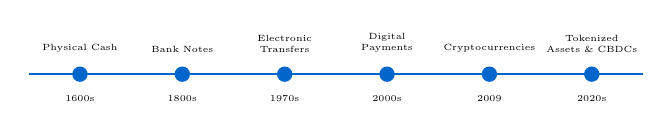
\begin{tikzpicture}[scale=0.65, transform shape]
    % Timeline
    \draw[thick, dfblue] (0,0) -- (12,0);

    % Points
    \foreach \x/\label/\year in {1/Physical Cash/1600s, 3/Bank Notes/1800s, 5/Electronic Transfers/1970s, 7/Digital Payments/2000s, 9/Cryptocurrencies/2009, 11/Tokenized Assets \& CBDCs/2020s} {
        \fill[dfblue] (\x,0) circle (0.15);
        \node[above, font=\tiny, text width=1.8cm, align=center] at (\x,0.3) {\label};
        \node[below, font=\tiny] at (\x,-0.3) {\year};
    }
\end{tikzpicture}
\end{center}

\vspace{0.3cm}
\textbf{Why Now?}
\begin{itemize}
    \item Blockchain provides programmable, trustless infrastructure
    \item COVID accelerated digital payment adoption globally
    \item Stablecoins demonstrated demand for digital dollars
    \item Central banks responding to private digital currency competition
\end{itemize}

\vspace{0.2cm}
\begin{block}{Market Context}
Boston Consulting Group projects \textbf{\$16 trillion} in tokenized assets by 2030---roughly the size of China's entire economy. Over \textbf{130 countries} are exploring CBDCs (research $\to$ pilot $\to$ limited launch $\to$ full launch).
\end{block}
\end{frame}

% =====================================================================
% SLIDES 5-24: CORE CONTENT
% =====================================================================
\begin{frame}{What is Tokenization?}
\begin{columns}[T]
\begin{column}{0.55\textwidth}
\begin{block}{Definition}
\textbf{Tokenization} is the process of creating a digital representation of a real-world asset on a blockchain.
\end{block}

\vspace{0.3cm}
\textbf{What Can Be Tokenized:}
\begin{itemize}
    \item Real estate
    \item Securities (stocks, bonds)
    \item Commodities (gold, oil)
    \item Art and collectibles
    \item Intellectual property
    \item Carbon credits
\end{itemize}
\end{column}

\begin{column}{0.42\textwidth}
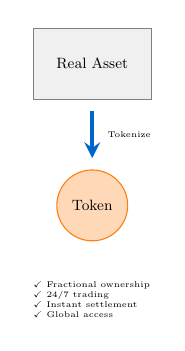
\begin{tikzpicture}[scale=0.6, transform shape]
    % Real asset
    \node[rectangle, draw=dfgray, fill=lightgray, minimum width=2.5cm, minimum height=1.5cm] (asset) at (0, 2.5) {};
    \node[font=\small] at (0, 2.5) {Real Asset};

    % Arrow
    \draw[arrow, line width=1.5pt] (0, 1.5) -- (0, 0.5);
    \node[right, font=\tiny] at (0.2, 1) {Tokenize};

    % Token
    \node[circle, draw=dforange, fill=dforange!30, minimum size=1.5cm] (token) at (0, -0.5) {};
    \node[font=\small] at (0, -0.5) {Token};

    % Benefits
    \node[font=\tiny, text width=2.5cm, align=left] at (0, -2.5) {
        $\checkmark$ Fractional ownership\\
        $\checkmark$ 24/7 trading\\
        $\checkmark$ Instant settlement\\
        $\checkmark$ Global access
    };
\end{tikzpicture}
\end{column}
\end{columns}
\end{frame}

\begin{frame}{Real-World Asset (RWA) Tokenization}
\begin{center}
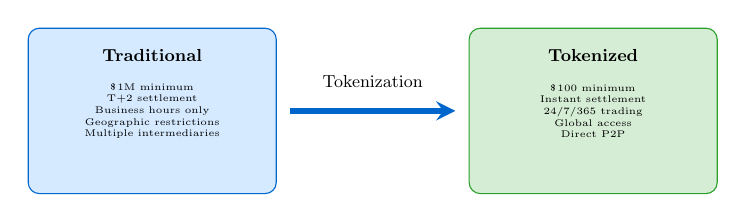
\begin{tikzpicture}[scale=0.7, transform shape]
    % Traditional
    \node[rectangle, draw=dfblue, fill=dflightblue4, minimum width=4.5cm, minimum height=3cm, rounded corners] (trad) at (-4, 0) {};
    \node[font=\small\bfseries] at (-4, 1) {Traditional};
    \node[font=\tiny, text width=4cm, align=center] at (-4, 0) {
        \$1M minimum\\
        T+2 settlement\\
        Business hours only\\
        Geographic restrictions\\
        Multiple intermediaries
    };

    % Arrow
    \draw[arrow, line width=2pt] (-1.5, 0) -- (1.5, 0);
    \node[above, font=\small] at (0, 0.3) {Tokenization};

    % Tokenized
    \node[rectangle, draw=dfgreen, fill=dfgreen!20, minimum width=4.5cm, minimum height=3cm, rounded corners] (tok) at (4, 0) {};
    \node[font=\small\bfseries] at (4, 1) {Tokenized};
    \node[font=\tiny, text width=4cm, align=center] at (4, 0) {
        \$100 minimum\\
        Instant settlement\\
        24/7/365 trading\\
        Global access\\
        Direct P2P
    };
\end{tikzpicture}
\end{center}

\vspace{0.3cm}
\textbf{Market Size Projections:}
\begin{itemize}
    \item Boston Consulting Group: \$16 trillion by 2030
    \item BlackRock, JP Morgan actively building infrastructure
    \item US Treasuries on-chain: \$1B+ (2024)
\end{itemize}
\end{frame}

\begin{frame}{Fractional Ownership: Democratizing Investment}
\begin{columns}[T]
\begin{column}{0.48\textwidth}
\textbf{The Problem:}
\begin{itemize}
    \item High-value assets require large capital
    \item Real estate: \$100K+ minimum
    \item Fine art: \$1M+ for blue-chip pieces
    \item Private equity: Accredited investors only
\end{itemize}

\vspace{0.3cm}
\textbf{The Solution:}
\begin{itemize}
    \item Divide asset into thousands of tokens
    \item Each token = proportional ownership
    \item Minimum investment: \$100 or less
    \item Receive proportional income/returns
\end{itemize}
\end{column}

\begin{column}{0.48\textwidth}
\begin{exampleblock}{Example: Tokenized Real Estate}
\textbf{Property Value:} \$1,000,000\\
\textbf{Total Tokens:} 10,000\\
\textbf{Price per Token:} \$100\\
\textbf{Monthly Rent:} \$5,000\\
\textbf{Your Investment:} 50 tokens (\$5,000)\\
\textbf{Your Monthly Income:} \$25
\end{exampleblock}

\vspace{0.2cm}
\textbf{Platforms:}
\begin{itemize}
    \item RealT, Lofty (real estate)
    \item Masterworks (art)
    \item Securitize (securities)
\end{itemize}
\end{column}
\end{columns}
\end{frame}

\begin{frame}{RWA Tokenization Examples}
\begin{center}
\footnotesize
\begin{tabular}{p{2.5cm}|p{2.8cm}|p{4cm}}
\toprule
\textbf{Asset Class} & \textbf{Platform} & \textbf{What They Do} \\
\midrule
Real Estate & RealT, Lofty & Buy fractions of rental properties starting at \$50; earn daily rent automatically \\
\addlinespace
US Treasuries & Ondo, Franklin Templeton & Invest in government bonds on-chain; earn ~5\% yield in your crypto wallet \\
\addlinespace
Private Credit & Centrifuge, Goldfinch & Access corporate loans normally reserved for institutions; 8-15\% yields \\
\addlinespace
Commodities & Paxos Gold (PAXG) & Each token = 1 oz gold in vault; trade 24/7 or redeem for physical bars \\
\addlinespace
Art & Masterworks & Own \$5M Banksy for \$100/share; platform handles storage, insurance, resale \\
\bottomrule
\end{tabular}
\end{center}

\vspace{0.3cm}
\begin{alertblock}{The Legal Challenge}
Tokens represent claims on assets, but enforcement still requires legal systems. ``Code is law'' doesn't apply when real-world assets need real-world courts.
\end{alertblock}
\end{frame}

\begin{frame}{Security Tokens vs. Utility Tokens}
\begin{columns}[T]
\begin{column}{0.48\textwidth}
\begin{block}{Security Tokens}
\textbf{Definition:} Digital representation of traditional securities
\begin{itemize}
    \item Represent ownership or economic rights
    \item Subject to securities regulations
    \item Provide dividends, profit sharing
    \item Require compliance (KYC/AML)
    \item Examples: tokenized stocks, bonds, real estate
\end{itemize}
\end{block}
\end{column}

\begin{column}{0.48\textwidth}
\begin{block}{Utility Tokens}
\textbf{Definition:} Access tokens for products/services
\begin{itemize}
    \item Provide access to platform functionality
    \item Generally not securities (but varies)
    \item No ownership or profit rights
    \item Used within specific ecosystems
    \item Examples: Filecoin, BAT, Chainlink
\end{itemize}
\end{block}
\end{column}
\end{columns}

\vspace{0.3cm}
\begin{alertblock}{The Howey Test (Plain English)}
US courts use 4 criteria to determine if something is a security: (1) investment of money, (2) in a common enterprise, (3) with expectation of profits, (4) from others' efforts. If all 4 apply, it's a security requiring SEC registration.
\end{alertblock}
\end{frame}

\begin{frame}{KYC/AML Regulatory Terms Explained}
\begin{columns}[T]
\begin{column}{0.48\textwidth}
\begin{block}{KYC (Know Your Customer)}
\textbf{What it means:} Financial institutions must verify who their customers are before providing services.
\begin{itemize}
    \item Collect government ID, address proof
    \item Screen against sanctions lists
    \item Understand customer's business
    \item Ongoing monitoring
\end{itemize}
\end{block}
\end{column}

\begin{column}{0.48\textwidth}
\begin{block}{AML (Anti-Money Laundering)}
\textbf{What it means:} Rules to prevent criminals from disguising illegally obtained money as legitimate income.
\begin{itemize}
    \item Monitor suspicious transactions
    \item Report large transactions (\$10K+ in US)
    \item Track source of funds
    \item File SARs (Suspicious Activity Reports)
\end{itemize}
\end{block}
\end{column}
\end{columns}

\vspace{0.3cm}
\textbf{Why it matters for tokenization:}
\begin{itemize}
    \item Security tokens require full KYC/AML compliance like traditional securities
    \item Tokenization platforms (Securitize, Polymath) automate compliance checks
    \item Trade-off: Privacy vs. regulatory legitimacy
\end{itemize}
\end{frame}

\begin{frame}{Tokenization Infrastructure: Key Players}
\begin{center}
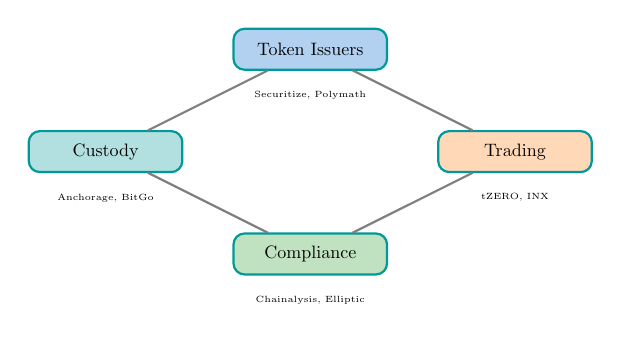
\begin{tikzpicture}[scale=0.65, transform shape]
    % Issuance layer
    \node[smartcontract, minimum width=3cm, fill=dfblue!30] (issuer) at (0, 2) {Token Issuers};
    \node[font=\tiny, below] at (0, 1.3) {Securitize, Polymath};

    % Custody layer
    \node[smartcontract, minimum width=3cm, fill=dfteal!30] (custody) at (-4, 0) {Custody};
    \node[font=\tiny, below] at (-4, -0.7) {Anchorage, BitGo};

    % Trading layer
    \node[smartcontract, minimum width=3cm, fill=dforange!30] (trading) at (4, 0) {Trading};
    \node[font=\tiny, below] at (4, -0.7) {tZERO, INX};

    % Compliance layer
    \node[smartcontract, minimum width=3cm, fill=dfgreen!30] (compliance) at (0, -2) {Compliance};
    \node[font=\tiny, below] at (0, -2.7) {Chainalysis, Elliptic};

    % Connections
    \draw[thick, dfgray] (issuer) -- (custody);
    \draw[thick, dfgray] (issuer) -- (trading);
    \draw[thick, dfgray] (custody) -- (compliance);
    \draw[thick, dfgray] (trading) -- (compliance);
\end{tikzpicture}
\end{center}

\textbf{Securitize and Polymath provide:}
\begin{itemize}
    \item Compliance automation (investor accreditation, KYC/AML)
    \item Token issuance smart contracts and cap table management
    \item Automated dividend distributions and regulatory reporting
    \item Secondary trading platforms
\end{itemize}
\end{frame}

\begin{frame}{Central Bank Digital Currencies (CBDCs)}
\begin{columns}[T]
\begin{column}{0.55\textwidth}
\begin{block}{Definition}
A \textbf{CBDC} is a digital form of central bank money, denominated in the national unit of account and a direct liability of the central bank.
\end{block}

\vspace{0.3cm}
\textbf{Global Status (2024):}
\begin{itemize}
    \item \textbf{130+ countries exploring}
    \item \textbf{Research:} Studying feasibility (US, UK)
    \item \textbf{Pilot:} Testing with users (China, India)
    \item \textbf{Limited launch:} Small-scale deployment (Nigeria)
    \item \textbf{Full launch:} Nationally available (Bahamas, Jamaica)
\end{itemize}
\end{column}

\begin{column}{0.42\textwidth}
\textbf{Two Main Types:}

\vspace{0.2cm}
\textbf{Retail CBDC:}
\begin{itemize}
    \item For general public
    \item Replaces/complements cash
    \item Direct central bank relationship
\end{itemize}

\vspace{0.2cm}
\textbf{Wholesale CBDC:}
\begin{itemize}
    \item For financial institutions
    \item Interbank settlements
    \item Less disruptive to banking
\end{itemize}
\end{column}
\end{columns}
\end{frame}

\begin{frame}{CBDC Architecture Models}
\begin{center}
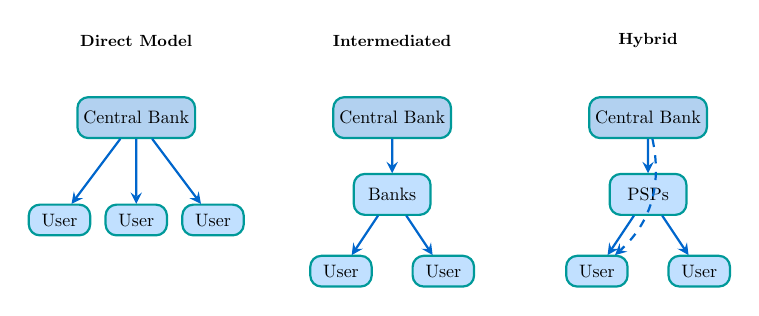
\begin{tikzpicture}[scale=0.65, transform shape]
    % Model 1: Direct
    \node[font=\small\bfseries] at (-5, 3) {Direct Model};
    \node[smartcontract, minimum width=2cm, fill=dfblue!30] (cb1) at (-5, 1.5) {Central Bank};
    \node[smartcontract, minimum width=1.2cm, minimum height=0.6cm] (u1a) at (-6.5, -0.5) {User};
    \node[smartcontract, minimum width=1.2cm, minimum height=0.6cm] (u1b) at (-5, -0.5) {User};
    \node[smartcontract, minimum width=1.2cm, minimum height=0.6cm] (u1c) at (-3.5, -0.5) {User};
    \draw[arrow] (cb1) -- (u1a);
    \draw[arrow] (cb1) -- (u1b);
    \draw[arrow] (cb1) -- (u1c);

    % Model 2: Intermediated
    \node[font=\small\bfseries] at (0, 3) {Intermediated};
    \node[smartcontract, minimum width=2cm, fill=dfblue!30] (cb2) at (0, 1.5) {Central Bank};
    \node[smartcontract, minimum width=1.5cm, fill=dflightblue3] (bank2) at (0, 0) {Banks};
    \node[smartcontract, minimum width=1.2cm, minimum height=0.6cm] (u2a) at (-1, -1.5) {User};
    \node[smartcontract, minimum width=1.2cm, minimum height=0.6cm] (u2b) at (1, -1.5) {User};
    \draw[arrow] (cb2) -- (bank2);
    \draw[arrow] (bank2) -- (u2a);
    \draw[arrow] (bank2) -- (u2b);

    % Model 3: Hybrid
    \node[font=\small\bfseries] at (5, 3) {Hybrid};
    \node[smartcontract, minimum width=2cm, fill=dfblue!30] (cb3) at (5, 1.5) {Central Bank};
    \node[smartcontract, minimum width=1.5cm, fill=dflightblue3] (psp) at (5, 0) {PSPs};
    \node[smartcontract, minimum width=1.2cm, minimum height=0.6cm] (u3a) at (4, -1.5) {User};
    \node[smartcontract, minimum width=1.2cm, minimum height=0.6cm] (u3b) at (6, -1.5) {User};
    \draw[arrow] (cb3) -- (psp);
    \draw[arrow, dashed] (cb3) to[bend left=30] (u3a);
    \draw[arrow] (psp) -- (u3a);
    \draw[arrow] (psp) -- (u3b);
\end{tikzpicture}
\end{center}

\vspace{0.2cm}
\textbf{Trade-offs:}
\begin{itemize}
    \item \textbf{Direct:} Maximum control, but central bank becomes retail bank
    \item \textbf{Intermediated:} Preserves banking system, but less innovative
    \item \textbf{Hybrid:} Balance, but complex implementation
\end{itemize}

\vspace{0.3cm}
\begin{block}{What Does This Mean for YOU?}
\textbf{Direct:} Bank at the Federal Reserve directly---your wallet is your Fed account\\
\textbf{Intermediated:} Keep using Chase/Wells Fargo, but your dollars are CBDCs behind the scenes\\
\textbf{Hybrid:} Choose either option depending on your needs (both available)
\end{block}
\end{frame}

\begin{frame}{Two-Tier CBDC Architecture}
\begin{center}
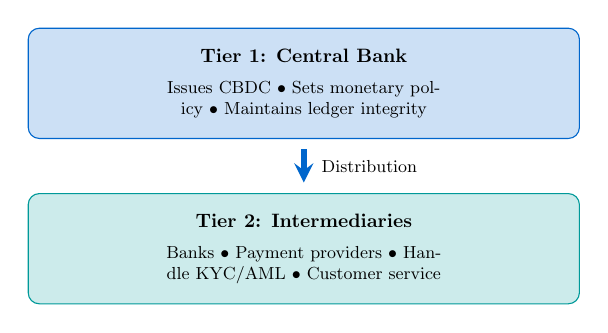
\begin{tikzpicture}[scale=0.7, transform shape]
    % Tier 1
    \node[rectangle, draw=dfblue, fill=dfblue!20, minimum width=10cm, minimum height=2cm, rounded corners] (tier1) at (0, 2) {};
    \node[font=\bfseries] at (0, 2.5) {Tier 1: Central Bank};
    \node[font=\small, text width=9cm, align=center] at (0, 1.7) {Issues CBDC $\bullet$ Sets monetary policy $\bullet$ Maintains ledger integrity};

    % Tier 2
    \node[rectangle, draw=dfteal, fill=dfteal!20, minimum width=10cm, minimum height=2cm, rounded corners] (tier2) at (0, -1) {};
    \node[font=\bfseries] at (0, -0.5) {Tier 2: Intermediaries};
    \node[font=\small, text width=9cm, align=center] at (0, -1.3) {Banks $\bullet$ Payment providers $\bullet$ Handle KYC/AML $\bullet$ Customer service};

    % Arrow
    \draw[arrow, line width=2pt] (0, 0.8) -- (0, 0.2);
    \node[right, font=\small] at (0.2, 0.5) {Distribution};
\end{tikzpicture}
\end{center}

\vspace{0.3cm}
\textbf{Why Two-Tier?}
\begin{itemize}
    \item Preserves existing financial system structure
    \item Central bank avoids retail banking operations
    \item Leverages private sector innovation for customer service
    \item Similar to how physical cash distribution works today
\end{itemize}
\end{frame}

\begin{frame}{CBDC vs. Stablecoin Comparison}
\begin{center}
\footnotesize
\begin{tabular}{p{3cm}|p{4.5cm}|p{4.5cm}}
\toprule
\textbf{Attribute} & \textbf{CBDC} & \textbf{Stablecoin} \\
\midrule
Issuer & Central bank (sovereign) & Private company \\
Liability & Central bank balance sheet & Private balance sheet \\
Legal Status & Legal tender & Private money \\
Backing & Full faith of government & Reserves (varies) \\
Programmability & Policy-controlled & Open/permissionless \\
Privacy & Policy-dependent & Pseudonymous (public chains) \\
Innovation Speed & Slow (government) & Fast (private) \\
Interoperability & National focus & Global by default \\
Risk Profile & Sovereign risk only & Counterparty + operational \\
\bottomrule
\end{tabular}
\end{center}

\vspace{0.2cm}
\begin{block}{Key Question}
Will CBDCs complement, compete with, or regulate away private stablecoins?
\end{block}
\end{frame}

\begin{frame}{Programmable Money: Opportunities}
\begin{columns}[T]
\begin{column}{0.48\textwidth}
\textbf{What Programmability Enables:}
\begin{itemize}
    \item Conditional payments
    \item Automatic tax withholding
    \item Stimulus with expiration dates
    \item Supply chain financing
    \item Smart contract integration
\end{itemize}

\vspace{0.3cm}
\textbf{Benefits:}
\begin{itemize}
    \item Financial inclusion for unbanked
    \item Reduced fraud and money laundering
    \item Efficient policy transmission
    \item New business models
    \item Real-time economic data
\end{itemize}
\end{column}

\begin{column}{0.48\textwidth}
\begin{exampleblock}{Example: Targeted Stimulus}
\textbf{Traditional:}
\begin{itemize}
    \item Send checks to all citizens
    \item No control over spending
    \item Slow distribution
\end{itemize}

\textbf{Programmable CBDC:}
\begin{itemize}
    \item Instant distribution
    \item Expires in 90 days
    \item Only spendable at local businesses
    \item Automatic for eligible recipients
\end{itemize}
\end{exampleblock}
\end{column}
\end{columns}
\end{frame}

\begin{frame}{Programmable Money: Concerns}
\begin{alertblock}{Privacy and Control Concerns}
\begin{itemize}
    \item \textbf{Surveillance:} Complete transaction visibility for governments
    \item \textbf{Control:} Money that can ``expire'' or be frozen remotely
    \item \textbf{Exclusion:} Programmable discrimination (restricting purchases)
    \item \textbf{Security:} Single point of failure for entire economy
\end{itemize}
\end{alertblock}

\vspace{0.3cm}
\textbf{Design Choices That Matter:}
\begin{itemize}
    \item \textbf{Token-based vs. Account-based:} Tokens offer more anonymity
    \item \textbf{Privacy-preserving technology:} Zero-knowledge proofs
    \item \textbf{Offline capability:} Works without internet
    \item \textbf{Holding limits:} Prevent bank disintermediation
    \item \textbf{Tiered privacy:} Small transactions anonymous, large ones tracked
\end{itemize}
\end{frame}

\begin{frame}{Privacy Design Spectrum}
\begin{center}
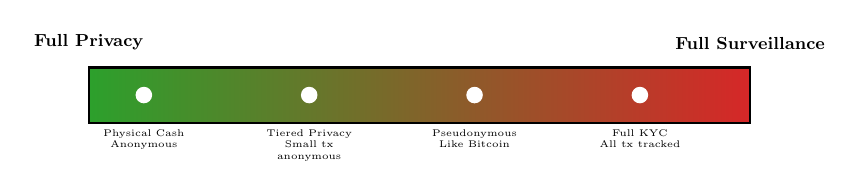
\begin{tikzpicture}[scale=0.7, transform shape]
    % Spectrum bar
    \draw[thick, left color=dfgreen, right color=dfred] (0,0) rectangle (12,1);

    % Labels
    \node[above, font=\small\bfseries] at (0,1.2) {Full Privacy};
    \node[above, font=\small\bfseries] at (12,1.2) {Full Surveillance};

    % Points on spectrum
    \node[below, font=\tiny, text width=2cm, align=center] at (1,0) {Physical Cash\\Anonymous};
    \node[below, font=\tiny, text width=2cm, align=center] at (4,0) {Tiered Privacy\\Small tx anonymous};
    \node[below, font=\tiny, text width=2cm, align=center] at (7,0) {Pseudonymous\\Like Bitcoin};
    \node[below, font=\tiny, text width=2cm, align=center] at (10,0) {Full KYC\\All tx tracked};

    % Markers
    \fill[white] (1,0.5) circle (0.15);
    \fill[white] (4,0.5) circle (0.15);
    \fill[white] (7,0.5) circle (0.15);
    \fill[white] (10,0.5) circle (0.15);
\end{tikzpicture}
\end{center}

\vspace{0.5cm}
\textbf{The Fundamental Tension:}
\begin{itemize}
    \item Governments want: AML/KYC compliance, tax enforcement, sanctions
    \item Citizens want: Financial privacy, freedom from surveillance
    \item Solution space: Technical privacy (ZK proofs) + legal limits on access
\end{itemize}

\begin{block}{Key Insight}
Privacy in CBDCs is a political choice, not a technical limitation. The technology exists for both full surveillance and full privacy.
\end{block}
\end{frame}

\begin{frame}{Offline CBDC Capability}
\begin{columns}[T]
\begin{column}{0.48\textwidth}
\textbf{Why Offline Matters:}
\begin{itemize}
    \item Physical cash works without infrastructure
    \item Disaster scenarios (hurricanes, earthquakes)
    \item Rural areas with poor connectivity
    \item Vulnerable populations without smartphones
    \item National security resilience
\end{itemize}

\vspace{0.3cm}
\textbf{Technical Approaches:}
\begin{itemize}
    \item Hardware wallets with local storage
    \item NFC-based peer-to-peer transfer
    \item Store-and-forward protocols
    \item Eventual consistency on reconnection
\end{itemize}
\end{column}

\begin{column}{0.48\textwidth}
\begin{exampleblock}{China's e-CNY Offline}
\begin{itemize}
    \item Hardware wallet cards
    \item NFC tap-to-pay without internet
    \item Limited offline balance
    \item Syncs when reconnected
    \item Tested in 2022 Olympics
\end{itemize}
\end{exampleblock}

\vspace{0.2cm}
\begin{alertblock}{Challenge}
Double-spending prevention is harder offline. Solutions involve cryptographic limits and periodic reconciliation.
\end{alertblock}
\end{column}
\end{columns}
\end{frame}

\begin{frame}{Global CBDC Landscape: China's e-CNY}
\begin{columns}[T]
\begin{column}{0.55\textwidth}
\textbf{Status (2024):}
\begin{itemize}
    \item 260+ million wallets created
    \item Billions in transaction volume
    \item Integrated with Alipay/WeChat Pay
    \item Tested in 2022 Beijing Olympics
\end{itemize}

\vspace{0.3cm}
\textbf{Key Features:}
\begin{itemize}
    \item Centralized architecture
    \item ``Controlled anonymity'' model
    \item Offline hardware wallet cards
    \item Programmable ``red packet'' gifts
    \item Cross-border pilots (Hong Kong, Thailand)
\end{itemize}
\end{column}

\begin{column}{0.42\textwidth}
\begin{block}{Design Philosophy}
\begin{itemize}
    \item Complement, not replace, existing payments
    \item Two-tier distribution via banks
    \item Central bank maintains ultimate control
    \item Privacy tiers based on wallet type
\end{itemize}
\end{block}

\vspace{0.2cm}
\textbf{Geopolitical Implications:}
\begin{itemize}
    \item Potential alternative to USD system
    \item Cross-border settlement without SWIFT
    \item First-mover advantage in CBDC standards
\end{itemize}
\end{column}
\end{columns}
\end{frame}

\begin{frame}{Global CBDC Landscape: Digital Euro}
\begin{columns}[T]
\begin{column}{0.55\textwidth}
\textbf{ECB Timeline:}
\begin{itemize}
    \item 2021: Investigation phase launched
    \item 2023: Preparation phase began
    \item Late 2020s: Potential launch
\end{itemize}

\vspace{0.3cm}
\textbf{Design Priorities:}
\begin{itemize}
    \item Privacy protection (transactions not visible to ECB)
    \item Offline capability
    \item Coexistence with physical cash
    \item Two-tier distribution through banks
    \item Holding limits to prevent bank runs
\end{itemize}
\end{column}

\begin{column}{0.42\textwidth}
\begin{block}{Key Concerns Addressed}
\begin{itemize}
    \item \textbf{Privacy:} Strong legal protections
    \item \textbf{Banks:} Won't disintermediate
    \item \textbf{Cash:} Complement, not replace
    \item \textbf{Control:} Democratic oversight
\end{itemize}
\end{block}

\vspace{0.2cm}
\textbf{Contrast with China:}
\begin{itemize}
    \item Slower, more deliberate approach
    \item Greater emphasis on privacy
    \item Democratic accountability
    \item Political approval required
\end{itemize}
\end{column}
\end{columns}
\end{frame}

\begin{frame}{Global CBDC Landscape: United States}
\begin{columns}[T]
\begin{column}{0.55\textwidth}
\textbf{Federal Reserve Position:}
\begin{itemize}
    \item Research and public consultation phase
    \item No commitment to issue CBDC
    \item Requires Congressional authorization
    \item Prioritizes careful deliberation over speed
\end{itemize}

\vspace{0.3cm}
\textbf{Key Concerns:}
\begin{itemize}
    \item Bank disintermediation risk
    \item Privacy protection
    \item Cybersecurity vulnerabilities
    \item Dollar's global reserve status
    \item Political controversy
\end{itemize}
\end{column}

\begin{column}{0.42\textwidth}
\begin{alertblock}{Political Divide}
\begin{itemize}
    \item \textbf{Supporters:} Financial inclusion, payment efficiency
    \item \textbf{Opponents:} Surveillance concerns, government overreach
\end{itemize}
\end{alertblock}

\vspace{0.2cm}
\textbf{Alternative Approach:}
\begin{itemize}
    \item Regulated stablecoins instead?
    \item FedNow instant payments (2023)
    \item Private sector innovation
    \item Watch and learn from others
\end{itemize}
\end{column}
\end{columns}
\end{frame}

\begin{frame}{Cross-Border CBDCs: mBridge}
\begin{columns}[T]
\begin{column}{0.55\textwidth}
\textbf{What is mBridge?}
\begin{itemize}
    \item Multi-CBDC platform by BIS Innovation Hub
    \item Participants: China, Hong Kong, Thailand, UAE, Saudi Arabia
    \item Enables direct central bank-to-central bank settlements
\end{itemize}

\vspace{0.3cm}
\textbf{Problems Solved:}
\begin{itemize}
    \item Correspondent banking is slow (days)
    \item High fees (3-5\% for remittances)
    \item USD intermediation required
    \item Limited operating hours
\end{itemize}
\end{column}

\begin{column}{0.42\textwidth}
\begin{block}{mBridge Benefits}
\begin{itemize}
    \item Instant, 24/7 settlement
    \item Direct currency exchange
    \item Lower transaction costs
    \item No USD intermediation
    \item Common technical platform
\end{itemize}
\end{block}

\vspace{0.2cm}
\textbf{Geopolitical Significance:}
\begin{itemize}
    \item Alternative to SWIFT
    \item Reduces dollar dominance
    \item New monetary architecture
\end{itemize}
\end{column}
\end{columns}
\end{frame}

\begin{frame}{The Tokenization Landscape}
\begin{center}
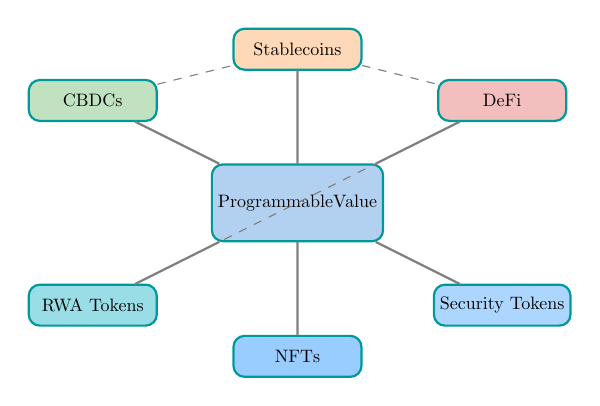
\begin{tikzpicture}[scale=0.65, transform shape]
    % Central concept
    \node[smartcontract, minimum width=3cm, minimum height=1.5cm, fill=dfblue!30] (center) at (0, 0) {Programmable\\Value};

    % Surrounding concepts
    \node[smartcontract, minimum width=2.5cm, fill=dfgreen!30] (cbdc) at (-4, 2) {CBDCs};
    \node[smartcontract, minimum width=2.5cm, fill=dforange!30] (stable) at (0, 3) {Stablecoins};
    \node[smartcontract, minimum width=2.5cm, fill=dfred!30] (defi) at (4, 2) {DeFi};
    \node[smartcontract, minimum width=2.5cm, fill=dfcyan!50] (rwa) at (-4, -2) {RWA Tokens};
    \node[smartcontract, minimum width=2.5cm, fill=dflightblue] (nft) at (0, -3) {NFTs};
    \node[smartcontract, minimum width=2.5cm, fill=dflightblue2] (sec) at (4, -2) {Security Tokens};

    % Connections
    \draw[thick, dfgray] (center) -- (cbdc);
    \draw[thick, dfgray] (center) -- (stable);
    \draw[thick, dfgray] (center) -- (defi);
    \draw[thick, dfgray] (center) -- (rwa);
    \draw[thick, dfgray] (center) -- (nft);
    \draw[thick, dfgray] (center) -- (sec);

    % Cross connections
    \draw[dashed, dfgray] (stable) -- (defi);
    \draw[dashed, dfgray] (rwa) -- (defi);
    \draw[dashed, dfgray] (cbdc) -- (stable);
\end{tikzpicture}
\end{center}

\textbf{The Convergence Thesis:} Traditional finance (TradFi) and decentralized finance (DeFi) are converging. The future is not ``either/or'' but hybrid systems combining the best of both.
\end{frame}

\begin{frame}{Legal and Regulatory Challenges}
\begin{columns}[T]
\begin{column}{0.48\textwidth}
\textbf{Token = Claim on Asset}
\begin{itemize}
    \item Blockchain state $\neq$ legal reality
    \item Smart contracts can't seize physical property
    \item Courts must enforce real-world claims
    \item Cross-jurisdictional complexity
\end{itemize}

\vspace{0.3cm}
\textbf{Key Challenges:}
\begin{itemize}
    \item Securities classification (Howey Test)
    \item Custody and private key management
    \item Settlement finality questions
    \item Investor protection requirements
\end{itemize}
\end{column}

\begin{column}{0.48\textwidth}
\begin{alertblock}{The Dual Reality Problem}
\textbf{Blockchain says:} Alice owns 100 tokens representing 1\% of building

\textbf{Legal question:} What happens when:
\begin{itemize}
    \item Alice loses her private key?
    \item The building is damaged?
    \item Local laws change?
    \item Token issuer goes bankrupt?
\end{itemize}
\end{alertblock}

\vspace{0.2cm}
\textbf{Solution:} Legal wrappers, regulated custodians, clear jurisdiction
\end{column}
\end{columns}
\end{frame}

% =====================================================================
% SLIDES 25-28: ADDITIONAL CONTENT (CASE STUDIES)
% =====================================================================
\begin{frame}{Case Study: Franklin Templeton On-Chain Fund}
\begin{columns}[T]
\begin{column}{0.55\textwidth}
\textbf{Background:}
\begin{itemize}
    \item Franklin Templeton: \$1.5T+ AUM
    \item Launched OnChain U.S. Government Money Fund
    \item First SEC-registered fund using blockchain
    \item Shares recorded on Stellar and Polygon
\end{itemize}

\vspace{0.3cm}
\textbf{How It Works:}
\begin{itemize}
    \item Fund invests in US government securities
    \item Each token = one share of fund
    \item Transfers settle on blockchain
    \item SEC-registered and compliant
\end{itemize}
\end{column}

\begin{column}{0.42\textwidth}
\begin{block}{Significance}
\begin{itemize}
    \item Major TradFi validates blockchain
    \item Regulatory approval achieved
    \item Real yield on-chain
    \item DeFi composability potential
\end{itemize}
\end{block}

\vspace{0.2cm}
\textbf{Lessons:}
\begin{itemize}
    \item Compliance is possible
    \item Hybrid models work
    \item Institutional adoption growing
    \item Infrastructure maturing
\end{itemize}
\end{column}
\end{columns}
\end{frame}

\begin{frame}{Case Study: Bahamas Sand Dollar}
\begin{columns}[T]
\begin{column}{0.55\textwidth}
\textbf{Background:}
\begin{itemize}
    \item First fully deployed retail CBDC (2020)
    \item Population: 400,000 across 700 islands
    \item Challenge: Banking access on remote islands
\end{itemize}

\vspace{0.3cm}
\textbf{Design Choices:}
\begin{itemize}
    \item Two-tier distribution through banks
    \item Mobile wallet-based
    \item Holding limits: \$500 (unverified), \$8,000 (verified)
    \item Transaction limits for privacy tiers
\end{itemize}
\end{column}

\begin{column}{0.42\textwidth}
\begin{block}{Results}
\begin{itemize}
    \item Improved financial inclusion
    \item Faster hurricane relief distribution
    \item Lower remittance costs
    \item Limited adoption (under 1\% of currency)
\end{itemize}
\end{block}

\vspace{0.2cm}
\textbf{Lessons Learned:}
\begin{itemize}
    \item Technology is the easy part
    \item Adoption requires incentives
    \item Education is critical
    \item Existing systems compete
\end{itemize}
\end{column}
\end{columns}
\end{frame}

\begin{frame}{Case Study: RealT Tokenized Real Estate}
\begin{columns}[T]
\begin{column}{0.55\textwidth}
\textbf{Platform Overview:}
\begin{itemize}
    \item Tokenizes US rental properties
    \item Minimum investment: \$50
    \item Daily rental income distribution
    \item Secondary trading on Uniswap
\end{itemize}

\vspace{0.3cm}
\textbf{Structure:}
\begin{itemize}
    \item Each property = separate LLC
    \item Tokens = LLC membership interests
    \item Smart contracts automate distributions
    \item Legal ownership via Delaware LLC
\end{itemize}
\end{column}

\begin{column}{0.42\textwidth}
\begin{block}{Benefits Demonstrated}
\begin{itemize}
    \item Global investors access US real estate
    \item Daily income (vs. monthly traditional)
    \item Transparent on-chain accounting
    \item 24/7 liquidity via DEXs
\end{itemize}
\end{block}

\vspace{0.2cm}
\textbf{Limitations:}
\begin{itemize}
    \item US accredited investors only (initially)
    \item Regulatory complexity
    \item Property management still needed
    \item Market risk remains
\end{itemize}
\end{column}
\end{columns}
\end{frame}

\begin{frame}{Case Study: Nigeria's eNaira Challenges}
\begin{columns}[T]
\begin{column}{0.55\textwidth}
\textbf{Background:}
\begin{itemize}
    \item Launched October 2021
    \item Africa's first CBDC
    \item Goal: Financial inclusion for 36M unbanked
\end{itemize}

\vspace{0.3cm}
\textbf{What Went Wrong:}
\begin{itemize}
    \item Only 0.5\% of population adopted (2023)
    \item Cash withdrawal limits to force adoption
    \item Public backlash and protests
    \item Trust deficit with government
\end{itemize}
\end{column}

\begin{column}{0.42\textwidth}
\begin{alertblock}{Key Lessons}
\begin{itemize}
    \item Can't force CBDC adoption
    \item Trust is prerequisite
    \item Cash restrictions backfire
    \item Infrastructure must exist
\end{itemize}
\end{alertblock}

\vspace{0.2cm}
\textbf{Contrast with Success:}
\begin{itemize}
    \item India's UPI (not CBDC) succeeded
    \item Voluntary adoption works better
    \item Incentives > mandates
    \item Build on existing behavior
\end{itemize}
\end{column}
\end{columns}
\end{frame}

% =====================================================================
% SLIDES 29-30: DISCUSSION/APPLICATION
% =====================================================================
\begin{frame}{Discussion: Should Central Banks Issue Retail CBDCs?}
\begin{columns}[T]
\begin{column}{0.48\textwidth}
\textbf{Arguments FOR:}
\begin{itemize}
    \item Preserve public money option as cash declines
    \item Financial inclusion for unbanked
    \item More efficient monetary policy
    \item Counter private stablecoin dominance
    \item Reduce payment system costs
    \item Enable programmable fiscal policy
\end{itemize}
\end{column}

\begin{column}{0.48\textwidth}
\textbf{Arguments AGAINST:}
\begin{itemize}
    \item Privacy and surveillance concerns
    \item Bank disintermediation risk
    \item Cybersecurity vulnerabilities
    \item Operational burden on central banks
    \item Existing systems work adequately
    \item Political weaponization risk
\end{itemize}
\end{column}
\end{columns}

\vspace{0.3cm}
\begin{block}{Discussion Questions}
\begin{itemize}
    \item Would you trust a government-issued digital currency?
    \item How should programmable money be governed?
    \item What privacy guarantees are non-negotiable?
\end{itemize}
\end{block}
\end{frame}

\begin{frame}{Application: Evaluating Tokenization Projects}
\begin{block}{Due Diligence Framework}
\begin{enumerate}
    \item \textbf{Legal Structure:} Does the token legally represent the claimed asset?
    \item \textbf{Custody:} Who holds the underlying asset? What happens if they fail?
    \item \textbf{Regulatory Compliance:} Is the offering properly registered?
    \item \textbf{Liquidity:} Can you actually sell the token when needed?
    \item \textbf{Audit Trail:} Are reserves/assets independently verified?
    \item \textbf{Jurisdiction:} Where would disputes be resolved?
\end{enumerate}
\end{block}

\vspace{0.3cm}
\textbf{Red Flags:}
\begin{itemize}
    \item Unclear legal structure or offshore entities
    \item No independent audits of underlying assets
    \item Promises of guaranteed returns
    \item No regulatory registration for securities-like tokens
\end{itemize}
\end{frame}

% =====================================================================
% SLIDE 31: EXECUTIVE SUMMARY
% =====================================================================
\begin{frame}{Executive Summary}
\begin{columns}[T]
\begin{column}{0.48\textwidth}
\textbf{Asset Tokenization:}
\begin{itemize}
    \item Creates digital representations of real assets
    \item Enables fractional ownership and 24/7 trading
    \item \$16T projected market by 2030
    \item Legal enforcement still requires courts
\end{itemize}

\vspace{0.3cm}
\textbf{CBDCs:}
\begin{itemize}
    \item Digital sovereign currency
    \item 130+ countries exploring
    \item Retail vs. wholesale types
    \item Design choices determine privacy
\end{itemize}
\end{column}

\begin{column}{0.48\textwidth}
\textbf{Key Trade-offs:}
\begin{itemize}
    \item Privacy vs. compliance
    \item Innovation vs. stability
    \item Inclusion vs. control
    \item National vs. global systems
\end{itemize}

\vspace{0.3cm}
\textbf{The Bottom Line:}
\begin{itemize}
    \item Programmable money is coming
    \item Design choices are political
    \item TradFi and DeFi converging
    \item Regulatory clarity emerging
\end{itemize}
\end{column}
\end{columns}
\end{frame}

% =====================================================================
% SLIDE 32: CONCEPT MAP
% =====================================================================
\begin{frame}{Concept Map: Tokenization and CBDCs}
\begin{center}
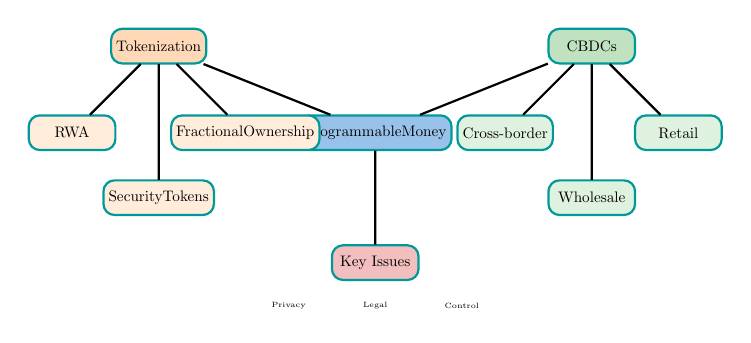
\begin{tikzpicture}[scale=0.55, transform shape]
    % Central node
    \node[smartcontract, minimum width=3cm, fill=dfblue!40] (prog) at (0,0) {Programmable\\Money};

    % Left branch - Tokenization
    \node[smartcontract, fill=dforange!30] (token) at (-5,2) {Tokenization};
    \node[smartcontract, minimum width=2cm, fill=dforange!15] (rwa) at (-7,0) {RWA};
    \node[smartcontract, minimum width=2cm, fill=dforange!15] (sec) at (-5,-1.5) {Security\\Tokens};
    \node[smartcontract, minimum width=2cm, fill=dforange!15] (frac) at (-3,0) {Fractional\\Ownership};

    % Right branch - CBDCs
    \node[smartcontract, fill=dfgreen!30] (cbdc) at (5,2) {CBDCs};
    \node[smartcontract, minimum width=2cm, fill=dfgreen!15] (retail) at (7,0) {Retail};
    \node[smartcontract, minimum width=2cm, fill=dfgreen!15] (whole) at (5,-1.5) {Wholesale};
    \node[smartcontract, minimum width=2cm, fill=dfgreen!15] (cross) at (3,0) {Cross-border};

    % Bottom - Concerns
    \node[smartcontract, fill=dfred!30] (concern) at (0,-3) {Key Issues};
    \node[font=\tiny] at (-2,-4) {Privacy};
    \node[font=\tiny] at (0,-4) {Legal};
    \node[font=\tiny] at (2,-4) {Control};

    % Connections
    \draw[thick] (prog) -- (token);
    \draw[thick] (prog) -- (cbdc);
    \draw[thick] (prog) -- (concern);
    \draw[thick] (token) -- (rwa);
    \draw[thick] (token) -- (sec);
    \draw[thick] (token) -- (frac);
    \draw[thick] (cbdc) -- (retail);
    \draw[thick] (cbdc) -- (whole);
    \draw[thick] (cbdc) -- (cross);
\end{tikzpicture}
\end{center}
\end{frame}

% =====================================================================
% SLIDES 33-34: KEY TERMS
% =====================================================================
\begin{frame}{Key Terms (1/2)}
\begin{description}
    \item[Tokenization] Creating digital blockchain representations of real-world assets
    \item[RWA] Real-World Assets - physical or traditional financial assets represented as tokens
    \item[Security Token] Token representing ownership in an asset, subject to securities laws
    \item[Utility Token] Token providing access to a product or service, not ownership
    \item[CBDC] Central Bank Digital Currency - digital sovereign money issued by central bank
    \item[Retail CBDC] Digital currency for general public use
    \item[Wholesale CBDC] Digital currency for financial institution settlements
    \item[Two-Tier Architecture] CBDC distributed through intermediaries, not directly by central bank
\end{description}
\end{frame}

\begin{frame}{Key Terms (2/2)}
\begin{description}
    \item[Programmable Money] Currency with embedded rules controlling spending/expiration
    \item[Fractional Ownership] Dividing asset ownership into small tradeable units
    \item[Interoperability] Ability of different digital currency systems to work together
    \item[mBridge] Multi-CBDC platform for cross-border central bank settlements
    \item[e-CNY] China's digital yuan CBDC
    \item[Digital Euro] ECB's planned CBDC for the Eurozone
    \item[Offline Capability] CBDC function without internet connectivity
    \item[Howey Test] Legal test determining if an asset is a security
\end{description}
\end{frame}

% =====================================================================
% SLIDE 35: COMMON MISCONCEPTIONS
% =====================================================================
\begin{frame}{Common Misconceptions}
\begin{columns}[T]
\begin{column}{0.48\textwidth}
\begin{alertblock}{Misconception 1}
``Tokenization eliminates all investment risks''
\end{alertblock}
\textbf{Reality:} Tokenization changes access and liquidity, not underlying asset risk. A tokenized building can still lose value.

\vspace{0.3cm}
\begin{alertblock}{Misconception 2}
``CBDCs are just like cryptocurrency''
\end{alertblock}
\textbf{Reality:} CBDCs are centralized, sovereign money. They share technology but not philosophy with decentralized crypto.
\end{column}

\begin{column}{0.48\textwidth}
\begin{alertblock}{Misconception 3}
``Code is law for tokenized assets''
\end{alertblock}
\textbf{Reality:} Physical assets require physical enforcement. Smart contracts can't seize a building---courts can.

\vspace{0.3cm}
\begin{alertblock}{Misconception 4}
``CBDCs will replace cash immediately''
\end{alertblock}
\textbf{Reality:} Most central banks plan CBDCs to complement, not replace cash. The ECB explicitly guarantees cash availability.
\end{column}
\end{columns}
\end{frame}

% =====================================================================
% SLIDES 36-37: SELF-ASSESSMENT QUESTIONS
% =====================================================================
\begin{frame}{Self-Assessment Question 1}
\begin{block}{Question (From Quiz 4.4, Q3)}
What is the primary benefit of fractional ownership through tokenization?
\end{block}

\begin{enumerate}[A)]
    \item It eliminates all investment risk
    \item It lowers barriers to entry by allowing investors to own small portions of high-value assets, democratizing access to investments previously limited to wealthy individuals
    \item It guarantees higher returns on investment
    \item It removes the need for legal contracts
\end{enumerate}

\vspace{0.5cm}
\pause
\textbf{Answer: B}

Fractional ownership enables multiple investors to own portions of high-value assets. Instead of needing \$1 million to buy a property, tokenization allows investments of \$100 or \$1,000 while maintaining liquidity through secondary trading.
\end{frame}

\begin{frame}{Self-Assessment Questions 2 \& 3}
\begin{block}{Q2 (Quiz 4.4, Q9): Direct vs. Intermediated CBDC Models}
In direct models, citizens hold accounts directly with the central bank; in intermediated models, commercial banks or PSPs manage customer relationships. \textbf{Answer: B}
\end{block}

\vspace{0.2cm}
\begin{block}{Q3 (Quiz 4.4, Q18): Tokenization Platforms}
Platforms like Securitize and Polymath provide infrastructure and compliance tools for issuing, managing, and trading security tokens in compliance with securities regulations. \textbf{Answer: B}
\end{block}

\vspace{0.3cm}
\textbf{Key Insights:}
\begin{itemize}
    \item Direct CBDC models create operational burden; intermediated models preserve banking roles
    \item Tokenization platforms bridge traditional securities law with blockchain technology
    \item Both represent the institutionalization of digital finance infrastructure
\end{itemize}
\end{frame}

% =====================================================================
% SLIDE 38: WHAT'S NEXT
% =====================================================================
\begin{frame}{What's Next: Day 5 Preview}
\begin{block}{Day 5: Risk and Regulation in Digital Finance}
\textbf{Topics to be covered:}
\begin{itemize}
    \item T5.1: Crypto market risks and volatility analysis
    \item T5.2: Smart contract security and audit frameworks
    \item T5.3: Global regulatory landscape (MiCA, SEC, international)
    \item T5.4: Compliance, AML/KYC, and institutional frameworks
\end{itemize}
\end{block}

\vspace{0.3cm}
\textbf{Connection to Today's Content:}
\begin{itemize}
    \item How are tokenized assets regulated differently from native crypto?
    \item What compliance requirements apply to security tokens?
    \item How do CBDCs fit into existing financial regulation?
    \item What risks are unique to programmable money?
\end{itemize}
\end{frame}

% =====================================================================
% SLIDE 39: RESOURCES
% =====================================================================
\begin{frame}{Resources for Further Learning}
\textbf{Academic \& Research:}
\begin{itemize}
    \item BIS Papers on CBDCs: \url{bis.org/cbdc}
    \item Atlantic Council CBDC Tracker: \url{atlanticcouncil.org/cbdctracker}
    \item ECB Digital Euro Documentation: \url{ecb.europa.eu/paym/digital_euro}
\end{itemize}

\vspace{0.3cm}
\textbf{Industry Reports:}
\begin{itemize}
    \item BCG ``Relevance of On-chain Asset Tokenization''
    \item McKinsey ``Tokenization: A Digital-Asset Deja Vu''
    \item World Economic Forum ``Digital Currency Governance Consortium''
\end{itemize}

\vspace{0.3cm}
\textbf{Tokenization Platforms:}
\begin{itemize}
    \item Securitize, Polymath (security tokens)
    \item RealT, Lofty (real estate)
    \item Ondo Finance (treasury tokens)
\end{itemize}
\end{frame}

% =====================================================================
% SLIDE 40: QUESTIONS
% =====================================================================
\begin{frame}{Questions?}
\begin{center}
\vspace{1cm}
{\Huge Topic 4.4: Tokenization and CBDCs}

\vspace{0.5cm}
{\large Digitizing Real-World Assets and Central Bank Digital Currencies}

\vspace{1cm}
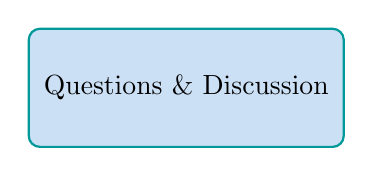
\begin{tikzpicture}
    \node[smartcontract, minimum width=4cm, minimum height=1.5cm, fill=dfblue!20] {Questions \& Discussion};
\end{tikzpicture}

\vspace{1cm}
\textbf{Next:} Day 5 -- Risk and Regulation in Digital Finance
\end{center}
\end{frame}

\end{document}
